 \section{Method}\label{methodology}
This section describes the methodology of the paper. First, in Section \ref{model}, the optimization model used is explained in detail. The focus is thereby on the mathematical formulation. However, where meaningful, qualitative explanations are added to give the reader a more complete understanding of the model. These qualitative explanations are used in particular to describe the main decision made by the model between maintaining operation, decommissioning or making replacement investment in existing gas grid pipelines. In Section \ref{gas_grid_austria}, the gas grid in Austria, which serves as the case study in this paper is presented. Then, in Section \ref{scenarios}, the four different scenarios are shown. Finally, Section \ref{data} provides information on the data used, while Section \ref{limitations} takes a critical look at the method and discusses some limitations and their impact on the results.
 
 \subsection{Optimization model}\label{model}
 
 
 \begin{figure}[h]
 	\centering
 	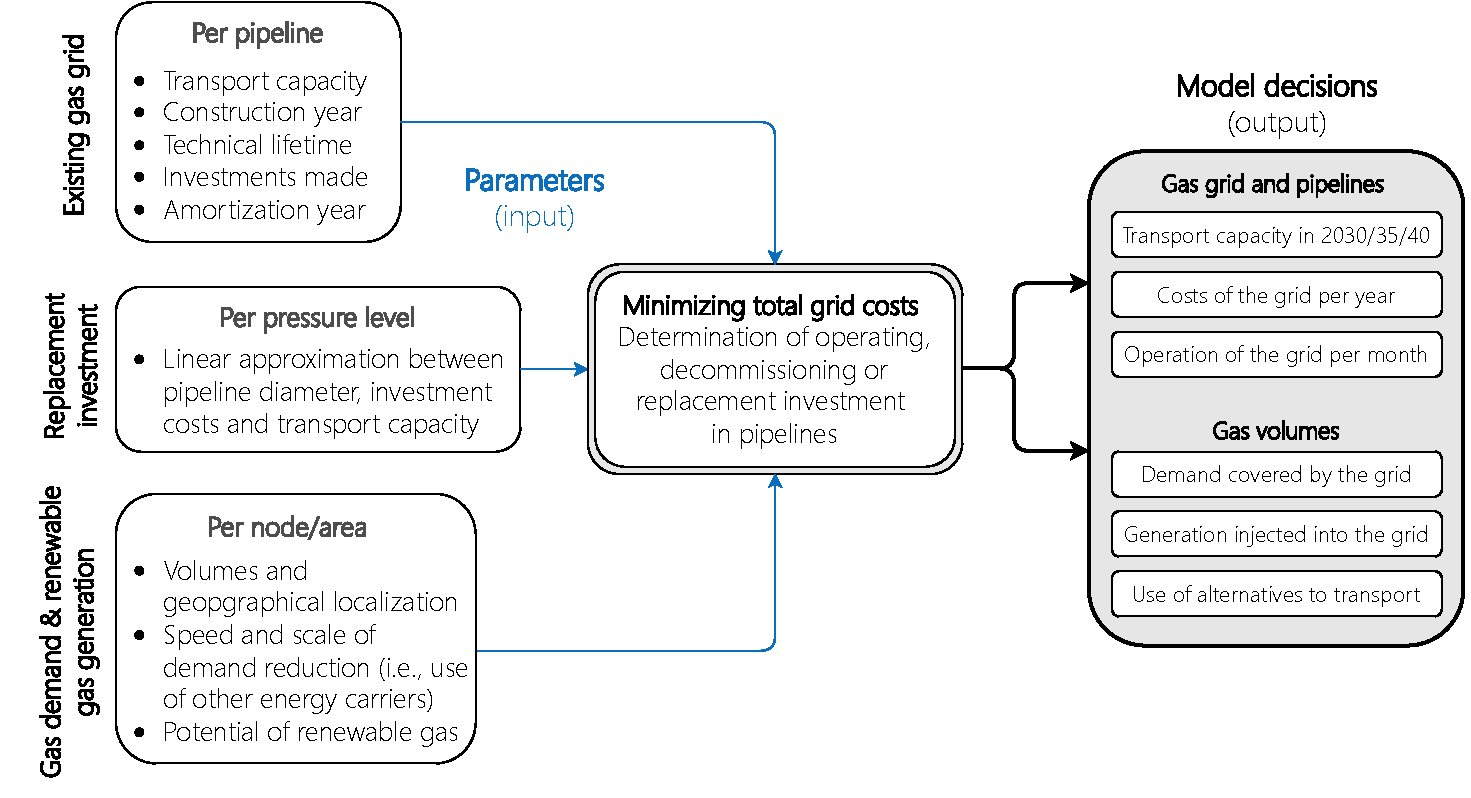
\includegraphics[width=1\linewidth]{figures/method/overview.pdf}
 	\caption{}
 	\label{}
 \end{figure}
 
 \subsubsection{Overview}
 
 % graphen basiertes model
 % schaut nur auf den energieträger gas
 % gas balance constraint per node
 
 % übersichtsgrafik was sind die inputs, was die outputs
 
 \subsubsection{Objective to minimize total grid costs}
 
 \subsubsection{Operation, decommissioning or replacement investment in pipelines}
 
 \subsubsection{Further constraints}
 
 

 

 
 
 

 \subsection{Existing gas grid in Austria}\label{gas_grid_austria}
 
 \subsection{Scenarios}\label{scenarios}
 
 \subsection{Data}\label{data}
 
 \subsection{Limitations}\label{limitations}
 % Schreiben dass es nicht zwingen notwendig sein muss holistisch darauf zu blicken
 
 % Druckniveaus
 % Umhängen von Verbrauch

 
 
 
 
 % 1) Optimierungsmodell
 	% 1.1 Übersicht über das Modell
 	% 1.2 Wesentlichen Funktionalitäten
 % 2) Szenarien
 	% Übersicht über die Szenarien 
 	% worin unterscheiden sich die Szenarien
 	% Detaillierte Beschreibung der Szenarien
% 3) Test-bed

 
 
 
 % vor dem ende der technischen lebensdauer
 % zum zeitpunkt des ablaufs der technischen lebensdauer
 
% This section explains the proposed methodology. First, Section \ref{Met:Intro} introduces the model. Then, Section \ref{Met:Equations} presents the mathematical formulation in detail. Section \ref{runs} explains the different model runs and defined scenarios. Section \ref{testbed} provides the test bed description and shows the gas networks in Vorarlberg, Austria, in detail, and Section \ref{label:inputs} presents the input data. Section \ref{label:limitation} discusses the limitations of the model. Finally, Section \ref{environment} deals with the open-source programming environment and the computation time of the model. 
% 
% \subsection{Introduction of the model}\label{Met:Intro}
% Figure \ref{fig:methodology} provides an overview of the method, including the interrelationships between the inputs (left), the \replaced{model}{modeling framework} (middle), and the outputs (right). Generally, the inputs (and thus parameters) can be divided into three different categories, namely, technical parameters (e.g., existing pipeline capacity per network/pressure level and the year of construction), economic parameters (e.g., refurbishment investment costs per pipeline), and further empirical data needs (e.g., gas demand and supply at the local community level and seasonal gas storage capacities). The \replaced[]{model}{modeling framework (CANCEL)} is developed as a linear program and is based on graph theory. It emphasizes the high spatial resolution in modeling. Particularly, a single node in the gas network graph corresponds to a community and covers an area of approximately \SI{40}{km^2} on average. The temporal resolution and thus investment planning horizon are until 2050, whereas an individual year is monthly resolved. \replaced[]{The model outputs include the optimal investment and dispatch decisions.}{Since the modeling framework is an investment and dispatch model, the outputs can also be divided into these catergories.} The outputs related to the investment decision are particularly the decommissioning and refurbishment investment decision per pipeline and gas network level. Additionally, the outputs encompass the dispatch of the gas networks on a monthly resolution. This includes the utilization of pipelines and particularly the gas demand and gas demand not supplied per community. 
% 
%  \begin{figure}[h]
% 	\centering
% 	\includegraphics[width=1\linewidth]{figures/flowchart.pdf}
% 	\caption{Overview of the method}
% 	\label{fig:methodology}
% \end{figure}
% 
% \subsection{Mathematical formulation}\label{Met:Equations}
% This section is dedicated to providing a detailed mathematical formulation of the \replaced[]{model}{modeling framework}. We start with the objective function and have deliberately chosen the further order of equations so that the following equation builds on the previous one as far as possible. \added[]{In addition to the detailed description of the equations below, Table} \ref{tab:brief} in \ref{app_overview} \added[]{summarizes the main equations of the model with a qualitative explanation.}\vspace{0.35cm}
% 
% Equation \ref{objective} shows the objective function of the model where $Capex$ is the net present value of the capital expenditures, $Opex$ of the operational expenditures, $Rev$ of the revenues from the supply of gas demands, and $Purch$ of purchasing gas. $Capex$ and $Opex$ represent the decommissioning and investment decision, whereas $Rev$ and $Purch$ the dispatch of the gas networks.  
% \begin{align}\label{objective}
%  	\underset{x}{\mathrm{min~}} Capex + Opex - Rev + Purch
%  \end{align}
%Additionally, $x$ represents the decision variables of the model. \added{All costs and prices are nominal.} Equation \ref{discount} shows the calculation of the discount factor per year $y$ ($\alpha_y$), where $i$ is the interest rate and $y_0$ is the reference year. 
%\begin{align}\label{discount}
%	\alpha_y = \frac{1}{(1+i)^{y-y_0}}
% \end{align}
%Building upon, $Capex$ is calculated as shown in Equation \ref{eq:capex} where $\omega$ is the weighted average cost of capital and $\Pi_y$ is the book value of the pipelines in $y$.
%\begin{align}\label{eq:capex}
%	Capex = \sum_{y}^{y_{end}-1} \alpha_y \cdot \omega \cdot \Pi_y + \underbrace{\alpha_{y_{end}} \cdot \Pi_{y_{end}}}_{\text{early depreciation}}	
%\end{align}
%Similarly, $Opex$ is calculated as shown in Equation \ref{eq:opex} where $\lambda_y$ is the fixed (operating) costs of the pipelines in $y$. 
%\begin{align}\label{eq:opex}
%	Opex = \sum_{y} \alpha_y \cdot \lambda_y
%\end{align}
%Equation \ref{eq:lambda} shows the calculation of the $\lambda_y$ where $c^{fix}_{l}$ is the specific fixed (operating) costs per $l$ and $\gamma_{l, y}$ is the installed pipeline capacity per $l$ in $y$.
%\begin{align}\label{eq:lambda}
%	\lambda_y = \sum_{l} c^{fix}_{l} \cdot \gamma_{l, y}
%\end{align}
%Equation \ref{eq:gamma} shows the calculation of $\gamma_{l, y}$ where $\gamma_{p,l,y}$ is the installed pipeline capacity at $p$ and $l$ in $y$ and $P_{l}$ the subset of all pipelines at $l$. \added[]{$\Lambda_{p}$ is a scaling factor. It is needed because the parameter $c^{fix}_{l}$ is defined for a representative pipeline length for each pressure level. These representative pipeline lengths are 50km and 25km for the high-pressure and mid-pressure network levels respectively. For example, if a pipeline $p$ at the high-pressure network level has a length of 50km, then the scaling factor $\Lambda_{p}$ is equal to 1. Note that $\Lambda_{p}$ is known a priori (because the length of pipelines are known) and is a parameter of the model.}
%\begin{align}\label{eq:gamma}
%	\gamma_{l, y} = \sum_{p \in P_{l}} \Lambda_{p} \cdot \gamma_{l, y, p}
%\end{align}
%Equation \ref{eq:total_capacity} defines the capacity of a pipeline $p$ at $l$ in $y$ where $\gamma^{pre}_{p,l,y}$ is the preexisting capacity and $\gamma^{ref}_{p,l,y}$ is the refurbished capacity of $p$ at $l$ in $y$. 
%\begin{align}\label{eq:total_capacity}
%	\gamma_{p,l, y} = \gamma^{pre}_{p,l,y} + \gamma^{ref}_{p,l,y}
%\end{align}
%Similarly, Equation \ref{eq:total_book_value} defines the book value of a pipeline $p$ at $l$ in $y$, where $\Pi^{pre}_{p,l,y}$ is the book value of the preexisting pipeline (capacity), $\Pi^{ref}_{p,l,y}$ of the refurbished capacity of $p$ at $l$ in $y$, and $f^{ref}_{p,l}$ the discount factor at $p$ and $l$.
%\begin{align}\label{eq:total_book_value}
%	\Pi_{p,l,y} = \Pi^{pre}_{p,l,y} + f^{ref}_{p,l} \cdot \Pi^{ref}_{p,l,y^{inv}_{p,l}}
%\end{align}
%Equation \ref{eq:tbv} sums the book values of all pipelines and network levels to obtain the total book value per $y$ ($\Pi_y$).
%\begin{align}\label{eq:tbv}
%	\Pi_{y} = \sum_{p} \sum_{l} \Pi_{p,l,y}
%\end{align}
%The following equation defines the refurbished installed capacity per $p$ at $l$ in $y$ resulting from the refurbishment (or decommissioning) decision in the year of the decision ($y^{inv}_{p,l}$).
%\begin{align}\label{9}
%	\gamma^{ref}_{p,l,y} = \begin{cases}
%		0 & \quad:\forall y~|~y<y^{inv}_{p,l}\\
%		\gamma^{ref}_{p,l,y-1} & \quad:\forall y~|~y>y^{inv}_{p,l}
%	\end{cases}
%\end{align}
%Equation \ref{eq:bvalue_ref} calculates the book value of the refurbishment investment at $p$ and $l$ in $y^{inv}_{p,l}$.
%\begin{align}\label{eq:bvalue_ref}
%	\Pi^{ref}_{p,l,y^{inv}_{p,l}} = c^{inv}_{l} \cdot \gamma^{ref}_{p,l,y^{inv}_{p,l}}
%\end{align}
%Equations \ref{exp} and \ref{imp} define the total gas export and import from $n$ at $l$ in $y$ and $m$ where $q_{p,l,y,m}$ is the amount of gas transported by $p$ at $l$ in $y$ and $m$. Additionally, $P^{exp}_{n,l}$ and $P^{imp}_{n,l}$ define the subsets containing all pipelines that can export and import gas from $n$ at $l$.
%\begin{align}
%	q^{exp}_{n,l,y,m} = \sum_{p \in P^{exp}_{n,l}} q_{p,l,y,m} \label{exp}\\
%	q^{imp}_{n,l,y,m} = \sum_{p \in P^{imp}_{n,l}} q_{p,l,y,m} \label{imp}
%\end{align}
%Equations \ref{bound1} and \ref{bound2} set the lower and upper bound of the amount of gas transported with respect to the installed pipeline capacity.
%\begin{align}
%	q_{p,l,y,m} \leq \gamma_{l, y, p} \label{bound1}\\
%	-q_{p,l,y,m} \leq \gamma_{l, y, p} \label{bound2}
%\end{align}
%The last two equations underline that a pipeline in the model has a certain direction in which the amount of gas transported is counted positively. Therefore, this direction defines for a node $n$ whether a pipeline $p$ is considered positively in the import or export balance (compare Equations \ref{exp} and \ref{imp}). Exemplarily, a pipeline $p$ could be considered in the export sum of a node $n$ on the one hand with a positive value if $p$ in fact exports gas from $n$ but on the other hand with a negative value if $p$ imports gas to $n$ in the dispatch of the model decision\footnote{We use this approach to prevent binary decision variables. Particularly, binary decision variables increase the computation time of graph-theory based models significantly. For more information, we refer to Kotzur et al. \cite{kotzur2021modeler} and their comprehensive review on how to handle complexity in energy system optimization.}.\vspace{0.35cm}
%
%Equation \ref{eq:balance} shows the general formulation of the balance constraint at $n$ where $q^{sto}_{n,l,y,m}$ is the amount of gas from or to storage. Particularly, this equation is defined for each network level $l$. The coupling of different network levels (e.g., the high- and mid-pressure network levels) is considered implicitly in the definition of the different gas demand variables (see Equation \ref{eq:demand} below). Additionally,  $\xi_m$ is a scaling (or transformation) factor that is defined for each month and is used to couple total values per month (e.g., $q^{dem}_{n,l,y,m}$) and peak values.\footnote{It reflects the fact that Equation \ref{eq:balance} encompasses variables that are associated with nodes ($q^{fed}_{n,l,y,m}$, $q^{dem}_{n,l,y,m}$, $q^{sto}_{n,l,y,m}$) modeled at a monthly resolution and with lines ($q^{exp}_{n,l,y,m}$, $q^{imp}_{n,l,y,m}$) modeled at a hourly resolution.}
%\begin{align}\label{eq:balance}
%	q^{fed}_{n,l,y,m} - q^{dem}_{n,l,y,m} - \xi_m \cdot \left(q^{exp}_{n,l,y,m} + q^{imp}_{n,l,y,m}\right) + q^{sto}_{n,l,y,m}= 0
%\end{align}
%Exemplarily, Equation \ref{eq:demand} shows the calculation of the gas demand at network level $l$, where $q^{del}_{n,l',y,m}$ is the amount of gas delivered from network level $l$ to $l'$ and $q^{dem,loc}_{n,l,y,m}$ is the local gas demand supplied at $n$. For example, $l$ could correspond to the transmission network level and $l'$ to the high-pressure network level. Note that the pressure in pipelines at $l$ is higher than at $l'$.
%\begin{align}\label{eq:demand}
%	q^{dem}_{n,l,y,m} = q^{dem,loc}_{n,l,y,m} + q^{del}_{n,l',y,m}
%\end{align}
%Equation \ref{eq:notsupplied} is the essential demand constraint and sets the upper bound of the decision variable $q^{dem,loc}_{n,l,y,m}$ to the maximum available gas demand $(d^{max}_{n,l,y,m})$, in which is defined as an input parameter. 
%\begin{align}\label{eq:notsupplied}
%	q^{dem,loc}_{n,l,y,m} \leq d^{max}_{n,l,y,m}
%\end{align}
%Particularly, Equation \ref{eq:notsupplied} allows the model by its mathematical operator with the less than or equal sign $(\leq)$ to decide between supplied and not supplied gas demand at the nodal level. This decision is in the foreground of the conducted analysis here, which is why we use particularly Equation \ref{eq:notsupplied} to define different model runs and thus scenarios. Accordingly, the model runs and scenarios differ by the individual specification of the demand constraint (i.e., $\leq$ or $=$ and $d^{max}_{n,l,y,m}$ as the upper bound of the equation). We refer to a detailed description of the model runs and scenarios in Section \ref{runs}.\vspace{0.3cm}
%
%The (total) quantity of gas fed at $l'$ is defined as stated in Equation \ref{eq:source} where $q^{fed,local}_{n,l',y,m}$ is the quantity of gas fed directly from $n$. 
% \begin{align}\label{eq:source}
% 	q^{fed}_{n,l',y,m} = q^{fed,local}_{n,l',y,m} + q^{del}_{n,l',y,m}
% \end{align}
%Equation \ref{eq:storage} defines the balance constraint of a storage unit. Contrary to most storage constraints, we do not consider different efficiency values for the charge and discharge. Hence, a single variable can be used. Additionally, $q^{sto,soc}_{n,l,y,m}$ is the state of charge. $\eta$ is the storage efficiency and thus models the losses with respect to the storage of gas between 2 months. 
%\begin{align}\label{eq:storage}
%		q^{sto,soc}_{n,l,y,m} = \eta \cdot q^{sto,soc}_{n,l,y,m-1} + q^{sto}_{n,l,y,m}
%\end{align}
%Equation \ref{eq:revenues} calculates the revenues created by the local gas demand supplied where $p^{loc}_{l,y}$ is the price. \added[]{The latter includes the gas price and the network charge.}
%\begin{align}\label{eq:revenues}
%	rev_{n,l,y,m} = p^{loc}_{l,y} \cdot q^{dem,loc}_{n,l,y,m}
%\end{align}
%Accordingly, the revenues ($Rev$ from the objective function in Equation \ref{objective}) are calculated as shown in Equation \ref{eq:total_revenues}.
%\begin{align}\label{eq:total_revenues}
%	Rev = \sum_{y} \sum_{n} \sum_{l} \sum_{m} \alpha_y \cdot rev_{n,l,y,m}
%\end{align}
%$Purch$ is calculated as shown in Equation \ref{eq:purchase}, where $p^{gas}_{y,m}$ is the gas price in $y$ and $m$. \added[]{As a result, the gas network operator only receives revenue through the network tariff. This becomes evident when comparing Equations \ref{eq:revenues} and \ref{eq:purchase}.}
%\begin{align}\label{eq:purchase}
%	Purch = \sum_{y} \sum_{n} \sum_{m} \alpha_y \cdot p^{gas}_{y,m} \cdot q^{del}_{n,l,y,m} \quad \text{with } l=\text{high-pressure}
%\end{align}
%Particularly, the influence of the gas price in the dispatch of gas networks is considered if gas is delivered from the transmission to the high-pressure network level. This is why Equation \ref{eq:purchase} is only defined for the high-pressure network level. This simplification is quite justified, first, because the gas storages, whose operation is significantly determined by the monthly gas price, are only present at the high pressure level, and second, because no gas delivery from the high pressure level to the transmission system is possible in the model. \added[]{The latter means that no delivery is possible from the distribution level (high-pressure and mid-pressure) to the transmission level.}
%
% \subsection{Model runs and defined scenarios}\label{runs}
% We conduct three different model runs, whereas each is associated with a scenario. Thereby, the model runs and defined scenarios differ in terms of consideration of the coverage of existing gas demands. Particularly, this is achieved by the modification and tailor-made adaption of the gas demand constraint in Equation \ref{eq:notsupplied}. As mentioned above, this emphasizes the model decision regarding the cost-optimal amount of gas demand supplied and not supplied. Table \ref{tabelle:modelruns} provides information for all model runs and associated scenarios related to the formulation/adaption of Equation \ref{eq:notsupplied}, the obtained gas network design, and the individual results. Note that the cost-optimal gas demand supplied $(\accentset{\ast}{\mathbf{q}}^{dem}_{n,l,y,m})$ without ensured supply (output of model run 1) is used as an input for model run 2 since it allows the tailor-made adaption of Equation \ref{eq:notsupplied} to assess the shadow price $\lambda^{CO}_{n,l,y,m}$ for the cost-optimal gas network without ensured gas supply. Similarly, model run 3 is used to obtain the shadow price $\lambda^{ES}_{n,l,y,m}$ in case of cost-optimality with an ensured supply of the gas network. 
%
%\begin{table}[h]
%\centering
%\resizebox{1\textwidth}{!}{% use resizebox with textwidth
%\renewcommand{\arraystretch}{2}
%\begin{tabular}{llll}
%	\toprule
%	\multicolumn{3}{c}{Input} & \multicolumn{1}{c}{Output}\\\cmidrule(lr){1-3}\cmidrule(lr){4-4}
%	\multirow{2}{*}{\makecell[l]{Model\\run}} & \multirow{2}{*}{\makecell[l]{Formulation of\\Equation \ref{eq:notsupplied}}} & \multirow{2}{*}{\makecell[l]{Scenario description/gas network design\\(abbreviation)}} & \multirow{2}{*}{\makecell[l]{Results or\\further used variable}}\\\\\hline
%	1 & $q^{dem}_{n,l,y,m} \leq d^{max}_{n,l,ym}$ & \multirow{2}{*}{Cost-optimal without ensured supply (CO)} & Demand supplied $(\accentset{\ast}{\mathbf{q}}^{dem}_{n,l,y,m})$\\
%	2 & $q^{dem}_{n,l,y,m} = \accentset{\ast}{\mathbf{q}}^{dem}_{n,l,y,m}$ & & Shadow price $(\lambda^{CO}_{n,l,y,m})$\\
%	3 & $q^{dem}_{n,l,y,m} = d^{max}_{n,l,ym}$ & Cost-optimal with ensured supply (ES) & Shadow price $(\lambda^{ES}_{n,l,y,m})$\\
%	\bottomrule
%	\end{tabular}}
%\caption{Model runs and associated formulation of the gas demand constraint (Equation \ref{eq:notsupplied}), scenarios, and results or further used variables.}
%\label{tabelle:modelruns}
%\end{table}
%
%\added[]{The different model runs and scenarios can also be viewed from the following perspective. Gas demand is assumed to decline by 2050 in all scenarios, regardless of whether ensured supply is taken into account or not. The remaining gas demand can therefore be considered as the gas demand of the so-called "hard-to-abate" energy services/sectors. In the case of ensured supply, the gas consumer is not disconnected. In order to quantify the network costs associated with ensured supply, we propose particularly the different model runs.}
%
%\subsection{Test bed description}\label{testbed}
%We illustrate the proposed model using the existing gas networks in Vorarlberg, Austria. Reasons for this test field include the fact that the gas networks there (i) are not connected to the rest of the Austrian gas network and can therefore be studied independently of it, (ii) include both high- and medium-pressure network levels that supply different energy services (e.g., heat for residential buildings, small and medium businesses (SMBs), and industry), and (iii) have cross-border pipelines to Germany and Liechtenstein. Therefore, the investigation of the Vorarlberg gas networks in this work can be seen as a reasonable balance between complexity and simplification against the background of a newly developed and to-be-tested model.
% 
% \subsubsection{Existing gas network in Vorarlberg, Austria}
% As mentioned above, the existing gas network in Vorarlberg, Austria, encompasses both a high- and a mid-pressure network. Particularly, the high-pressure network level includes a cross-border pipeline to Germany and Liechtenstein. \added[]{In this particular case, it is difficult to distinguish between the transmission level and the high pressure network level. Normally, the distinction could be made on the basis of the different pressure levels. However, as described above, the cross-border connections to Germany and Liechtenstein have similar pressure levels to the other high-pressure pipelines. We have therefore made the following assumptions. Since gas imports come from Germany and are transported to Liechtenstein through the Testbed network, we assume that the connection from the Testbed to Germany is the only pipeline at transmission level. The remaining pipelines are then part of the high and medium pressure level and therefore at distribution network level.} Table \ref{tab:summary_vorarlberg_network} provides a summary of Vorarlberg's gas network. The list of general indicators encompasses information related to the gas network, demand, and supply. Figure \ref{fig:comparison} shows the existing gas networks (left) and their representation in the model (right) in Vorarlberg, Austria. The high-pressure network level is comparatively well represented (difference of only \SI{3}{km} or less than 4\%). Nevertheless, the mid-pressure network level is underrepresented in the model. This issue is further processed in Sections \ref{label:inputs}, where we present the input data, and Section \ref{label:limitation}, where we discuss limitations of the model. In summary, Vorarlberg's gas networks are represented in the model by 36 nodes and 43 individual pipelines. \added[]{The single pipeline at the transmission network level, which is connected to node at the very top, is not explicitly shown.}
%  
%\begin{table} \centering
%	\resizebox{0.8\textwidth}{!}{
%		\renewcommand{\arraystretch}{1.3}
%		\begin{tabular}{ll}
%			\toprule 
%			\multicolumn{2}{l}{List of general indicators}\\\hline
%			Number of communities supplied & 39\\
%			Number of end-user systems & \SI{32615}{}\\
%			Gas supply within Vorarlberg, Austrian & \SI{2098}{GWh \per year}\\
%			Transmision to Liechtenstein & \SI{644}{GWh \per year}\\
%			Number of \replaced[]{biomethane}{green gas} production facilities & 2\\
%			Total green gas production & \SI{6,4}{MWh \per year}\\
%			Length of high-pressure network & \SI{83}{km}\\
%			Length of mid- and low-pressure network & \SI{2128}{km}\\
%			\bottomrule
%	\end{tabular}}
%	\caption{Summary of Vorarlberg's gas network, demand, and supply in 2020. Source: \cite{VorarlbergNetz2021}.}
%	\label{tab:summary_vorarlberg_network}
%\end{table}
%
%\begin{figure}[h]
%	\centering
%	\includegraphics[width=0.8\linewidth]{figures/Comparison.eps}
%	\caption{Existing gas networks (high-pressure in red and mid-pressure in green) in Vorarlberg, Austria (left), and its representation in the model (right). Source: \cite{VorarlbergNetz2021}.}
%	\label{fig:comparison}
%\end{figure}
% 
% \subsubsection{Gas demand decline pathways at the community level until 2050}
%This section is dedicated to describing the assumptions regarding the development of gas demands at the community level in Vorarlberg, Austria, until 2050. In a first step, we assess total gas demands at the community level in 2018 using information from the open data platform \textit{energiemosaik} \cite{energiemosaik} and our own database (see Section \ref{environment} for data availability). \added[]{Details of the current natural gas demand in Vorarlberg, Austria, is given in} \ref{app_demand}. In a second step, we use the classification of communities regarding the energy demand provided by energiemosaik to estimate the composition of local gas demands. Accordingly, the local gas demand in the community is allocated to one or more of the following sectors of end-use or items: residential, agriculture, industry, SMB, service, and mobility. Building upon this characterization of gas demands by items, the following claim is made: 
%
%\begin{addmargin}[0.75cm]{0pt}
%	The composition of the local gas demand at the community level in 2018 determines its development until 2050. Each sector of end-use/item is associated with a decline pathway until 2050. Thus, the total gas demand at the community level until 2050 is described by a linear combination of the individual decline pathways per sector of end-use.
%\end{addmargin}
%\vspace{0.35cm}
%
%Table \ref{tab:decline_pathway} shows the assumed annual decline rate (and thus decline pathway until 2050) per sector of end-use. We use the naming convention from energiemosaik and use the names Type A, B, C, and D for a combination of different sectors of end-use. We restrict ourselves to four different types (A-D) only. Note that 2050's share in gas demands are rough estimates including higher values if industry and SMBs are located there. For the residential/building heat demand, a linear decrease until 2040 is assumed. 
%\begin{table} \centering
%	\resizebox{1\textwidth}{!}{
%		\renewcommand{\arraystretch}{1.3}
%		\begin{tabular}{lccccr}
%			\toprule 
%			Name & Residential & Industry & SMB & Service &  Decline rate (2050's share)\\\hline
%			Type A & \checkmark & & & & Linear until 2040\\
%			Type B & \checkmark & \checkmark & \checkmark & & Linear (15\%)\\
%			Type C &  &  &  & \checkmark & Linear (20\%)\\
%			Type D &  & \checkmark &\checkmark & & Linear (35\%)\\
%			\bottomrule
%	\end{tabular}}
%	\caption{Annual decline rates for different compositions of gas demands at the local community level under the naming convention and sectors of end-use from energiemosaik \cite{energiemosaik}.}
%	\label{tab:decline_pathway}
%\end{table} 
%
%\subsubsection{Assumptions on the share of green gases in supply and network}
%
%\added{For the modeling it is necessary to estimate the share of green gases up to 2050. In general, this includes the supply of synthetic gas, biomethane and hydrogen. All three are subject to considerable uncertainty. In the Austrian discussion on biomethane and hydrogen, there is a consensus that hydrogen will not be added to natural gas. All national considerations of the gas and hydrogen network infrastructure follow the concept of two separate networks. We take this into account and therefore assume that there are no shares of hydrogen (i.e., no blending of hydrogen) and in the natural gas network. It is therefore not necessary in our specific case to consider the previously mentioned technical limits of hydrogen shares in gas networks. In general, however, such analyses must take into account the technical limits on hydrogen shares. For biomethane, the situation is different compared to hydrogen. It can be assumed that biomethane will be added to natural gas and transported through the gas network. Moreover, it is already added today (see the number of biomethane production facilities in Table \ref{tab:summary_vorarlberg_network}). However, it is uncertain whether large-scale biomethane production in Austria will be profitable in the future. We decide to make a rather conservative estimate of the future production of biomethane within the analyzed network. We assume a threefold increase in production from 2020 to 2030 and a constant remaining production thereafter. We discuss again the role of biomethane within the limitations of the model.}
%
% \subsection{Data}\label{label:inputs}
% This section shows \deleted{a selection of }the most relevant input data. \added{To replicate the present results, we refer to the code of the model in} \cite{Zwickl_Bernhard_Gas_network_decommissioning_2022} and the dataset at Zenodo \cite{zwicklbernhard_zenodo}. At the same time, we refer to the authors' GitHub repository (details in Section \ref{environment}) for the complete input data. Table \ref{tab:input_costs} shows the cost assumptions for gas networks including the specific investment costs ($c^{inv}_l$) and fixed costs per year ($c^{fix}_l$) for the different gas network levels. Note that 2030 is the assumed year of the decommissiong and refurbishment investment decision for all pipelines within the networks. Additionally, the development of natural gas prices in Europe is taken from the World Energy Outlook 2021 \cite{weoutlook}. The values from the so-called Stated Policies Scenario are taken: \SI{26.28}{EUR \per MWh} in 2030 and \SI{28.33}{EUR \per MWh} in 2050.\footnote{Assuming a linear development between 2030 and 2050.} Revenues are generated in this work on the basis of gas network usage fees. Accordingly, we assume the following values for $p^{loc}_{l,y}$ for each year: \SI{1}{EUR \per MWh} (high-pressure) and \SI{20}{EUR \per MWh} (mid-pressure).\footnote{Note that the currently high natural gas prices are not explicitly considered. However, it can be argued that they are implicitly included as an additional driver for the assumed declining gas demand rates.} 
% 
%\begin{table}[h]\centering
%	\resizebox{1\textwidth}{!}{
%	\renewcommand{\arraystretch}{1.3}
%	\begin{tabular}{lllrr}
%		\toprule 
%		Type of costs & Symbol & Network level ($l$) & Value & Source\\\hline
%		\multirow{3}{*}{\makecell[l]{Specific investment costs\\(used in Equation \ref{eq:bvalue_ref})}} & \multirow{3}{*}{$c^{inv}_l$} & Transmission & \SI{4600}{EUR\per MW\per km} & \cite{acer}\\
%		& & High-pressure & \SI{4000}{EUR\per MW\per km} & \multirow{2}{*}{\cite{EEG}}\\
%		& & Mid-pressure & \SI{3000}{EUR\per MW\per km} & \\\hline
%		\multirow{3}{*}{\makecell[l]{Fixed costs per year\\(used in Equation \ref{eq:lambda})}} & \multirow{3}{*}{$c^{fix}_l$} & Transmission & \multirow{3}{*}{\SI{2000}{EUR\per MW}} & \multirow{3}{*}{\cite{EEG}}\\ 
%		& & High-pressure & & \\
%		& & Mid-pressure & & \\
%		\bottomrule
%	\end{tabular}}
%\caption{Cost assumptions of gas networks. The value of specific investment costs of the mid-pressure network level is scaled by the ratio between the existing and the modeled pipeline length (as shown in Figure \ref{fig:comparison}).}
%\label{tab:input_costs}
%\end{table}
%
%\subsection{Limitation of the model}\label{label:limitation}
%Below, we discuss two different limitations of the model, whereas both can be associated with the trade-off decision between (spatial and temporal) granularity and computation time of the model. Besides, nonlinear hydraulic constraints and the book values of compressor stations are not considered.   
%
%\subsubsection{Under-representation of mid-pressure networks and related pipelines}
%With an eye on the representation of the mid-pressure gas network presented in Figure \ref{fig:comparison}, it is evident that the corresponding pipelines of the mid-pressure network level are underrepresented in the model. The main reason for this is the (limited) spatial granularity at the community level since large parts of the mid-pressure network are within communities. Within the simplification of the geometry of gas pipelines to the spatial granularity on a community level, mid-pressure gas pipelines within a single community are not considered. This is why the introduction of a tailor-made scaling factor is needed to adjust the specific refurbishment investment costs ($c^{inv}_{mid-pressure}$) accordingly (see Table \ref{tab:input_costs} in Section \ref{label:inputs}). Exemplarily, this scaling factor is $\frac{225}{97}$ (on average) in the case of the mid-pressure network level in Figure \ref{fig:comparison}. 
%
%\subsubsection{Resolution on a monthly basis and associated necessary scaling factors to calculate peak pipeline capacities}
%The temporal granularity of the model is limited since it generates results monthly within an individual year. Consequently, again, a scaling factor is needed to link the nodal gas balance constraints (monthly values) with the calculation of needed peak pipeline capacities (Equation \ref{eq:balance}). An hourly resolution could eliminate this calculation process, but, at the same time, one could run into serious computation time matters as the number of equations (i.e., gas balance constraints for node and network level) increases significantly. 
%
%\subsubsection{Assumptions on profitability and volumes of biomethane in the network}
%\added[]{Developments in gas demand and biomethane injection are assumed to be exogenous. Both are very difficult to estimate in the context of decarbonizing energy systems. Regarding the assumptions made for natural gas demand, at least the different model runs proposed in this work could increase the significance of the results, as the different model runs can be interpreted as a sensitivity analysis of the gas demand. For the biomethane production and injection into the network, this work assumes conservative volumes as described above. The impact of this assumption on the results is likely to vary between the different model runs proposed here. It depends on how gas demand is treated within the network. In the case of ensured supply (model run 3), therefore, only the network utilization is likely to be overestimated. This is because in this case, a area-wide network remains and biomethane could simply be integrated into the network. Due to the usually shorter distances between biomethane production and demand, this could reduce the network utilization (for example, by comparing the product of transported volumes and distance in} $GWh \cdot km$\added{). In the case without ensure supply (model runs 1 and 2), the biomethane assumption is likely to underestimate the size of the gas network and the volumes transported, as biomethane can be a driver for the use of gas networks. However, in our specific case, this aspect is likely to be small. Two reasons underline this viewpoint. First, as mentioned above, biomethane is usually produced and consumed locally. The transport over long distances is not reasonable mainly due to economic reasons. It would usually require recompression of the biomethane, which, depending on the pressure levels, is energy intensive and therefore very costly. In addition, the model would only underestimate the size of the gas network if biomethane production is higher than gas demand within a node in the network. Essentially, the network only sees the net demand of the node, which is the total demand minus the source. However, it is worth noting that biomethane injection can generally trigger investments in gas networks to enable connection.}
%
%\subsection{Open-source environment and calculation time}\label{environment}
%The developed optimization model is implemented in Python 3.8.12 using \deleted[]{the modeling framework} Pyomo version 5.7.3 \cite{hart2017optimization}. It is solved with the solver Gurobi version 9.0.3. For planning the development of gas networks in Vorarlberg, Austria, the model consists of 124155 equations and 98610 continuous variables. It takes on average \SI{3}{\second} to be solved using a computer with an Intel Core i7-8565U with 16 GB of RAM running Microsoft Windows 10 Pro with 64 bit. We use for data analysis the common data format template developed by the Integrated Assessment Modeling Consortium using the open-source Python package pyam \cite{huppmann2021pyam}. Note that all materials used in this study are disclosed as part of the publication on GitHub (\url{https://github.com/sebastianzwickl}). We refer to the repository for the codebase, data collection, and further information.